\chapter{Introduction}
Radiology is a powerful tool to detect and diagnose abnormalities by allowing doctors to visually inspect internal pathology that could not otherwise be seen. By virtue of integrating a ubiquitous medical practice with sophisticated engineering, the field has traditionally been at the forefront of medical technology. Digital radiology and picture archiving and communications systems led to an early, widespread adoption of electronic records with respect to imaging \cite{Strickland:2000cv,Bryan:1999kn}.

Despite the early adoption of computational systems to manage data, the actual practice of radiology remains a relatively unchanged. The doctor must still visually scan, detect, and interpret the findings in the image to deliver an impression. An unfortunate consequence of such a system is substantial variability in practice and performance \cite{Robinson:1997uq,Fitzgerald:2001hn}. This is not to say that radiologists are the only doctors faced with these issues, as the now infamous Institute of Medicine report \emph{To Err is Human: Building a Safer Health System} revealed a striking amount of poor patient outcomes are a result of medical error \cite{Anonymous:2000va}. As a motivating example, mammography, which has a tightly controlled terminology and strict standards of practice, has revealed substantial variability with regard to sensitivity and specificity of evaluation of lesion malignancy amongst different readers as well as different facilities \cite{Jackson:2009fw, Beam:1996ui, Elmore:2002vc, Taplin:2008bv}. Such variability is not restricted to diagnosis and impressions; even the \emph{findings} within the contents of the report have shown substantial variability \cite{Hobby:2000th, Robinson:1997uq}.

Decision Support Systems (DSS) have been developed to improve upon mammography interpretation and diagnosis \cite{Garg:2005cb, Burnside:2000wl, ElizabethS:2005gc, Rubin:2005jg}. DSS are tools that incorporate medical information to provide meaningful input to medical practitioners. However, to date, adoption of DSS has limited as they often interrupt the radiological workflow \cite{Morgan:2011ct}. In addition, decision support has only focused on diagnosis and automated computational analysis of image data. There has been little work using DSS to improve consistency and completeness of mammographic reporting, which ultimately would be important for improving radiologist diagnostic accuracy in assessing lesions on mammography.

The mammography report is of crucial importance, since it conveys the radiologist findings, interpretation of those findings in terms of likelihood of malignancy, and suggested patient management, such as follow-up imaging or biopsy. However, a major barrier is the inherent qualitative nature of current reporting practices which results in variation in practice and non-standard quality of patient care. Prior studies have shown the importance of good reporting practices and identified several key traits of good reports: correctness of findings, completeness of the description of significant clinical findings, consistency of report language and findings, and timeliness of the report's completion \cite{Johnson:2004kh, HaraldO:2004hi}. Variability in the report directly hampers the utility of mammographic diagnosis. False positives and defensive medical decision making cause patient anxiety, excessive additional invasive testing (e.g., biopsy), and rising healthcare costs, while false negatives result in delayed treatment at the expense of patient health.

The most headway in improving reporting content is in the field of mammography. Efforts to improve upon consistency and clarity of report language include the Breast Imaging-Reporting and Data System (BI-RADS) which provides a standard lexicon of descriptors for radiological observations \cite{Liberman:ws}. Additionally, Structured Reporting Systems have been designed to improve the quality of radiology reporting by providing templates with standardized information and support for BI-RADS \cite{Reiner:2009ib}. Unfortunately, structured reporting is generally more time-intensive and imposes distractions in the traditional radiological workflow, directly interfering with timeliness \cite{Weiss:2008er}. Moreover, these two approaches mainly aim to improve upon reporting language and clarity, not analyze report content. To this effect, 

Our hypothesis is that improving the correctness, consistency, and completeness of radiology reports can improve the sensitivity and specificity of diagnosis and thereby improve the quality of patient care. To tackle this challenge and to enable translation of DSS into clinical practice to benefit patient care, we propose a real-time DSS that provides feedback to radiologists as they generate their reports. This system will create evaluate and improve upon the content of a structured radiological report. This differs from traditional approaches to DSS because our system will improve upon reporting, and by our hypothesis, implicitly improve upon practice. By ensuring that the relevant observations are correctly, completeley, and consistently described in mammography reports, our DSS will reduce variability in practice, improving practitioner decision making and lead to better patient care.

\section{FASR: Fast Adaptive Structured Reporting}
The Fast Adaptive Structured Reporting (FASR) system's goal is to reduce variability and error in radiological interpretation by providing decision-support during reporting time. This works by incorporating multiple checks during the reporting process and providing real-time feedback to the radiologist.

There are three main components to FASR: (1) Verification of the annotation correctness, (2) assessment of report completeness, and (3) providing feedback to the radiologist.

\begin{figure}[h]
	\centering
	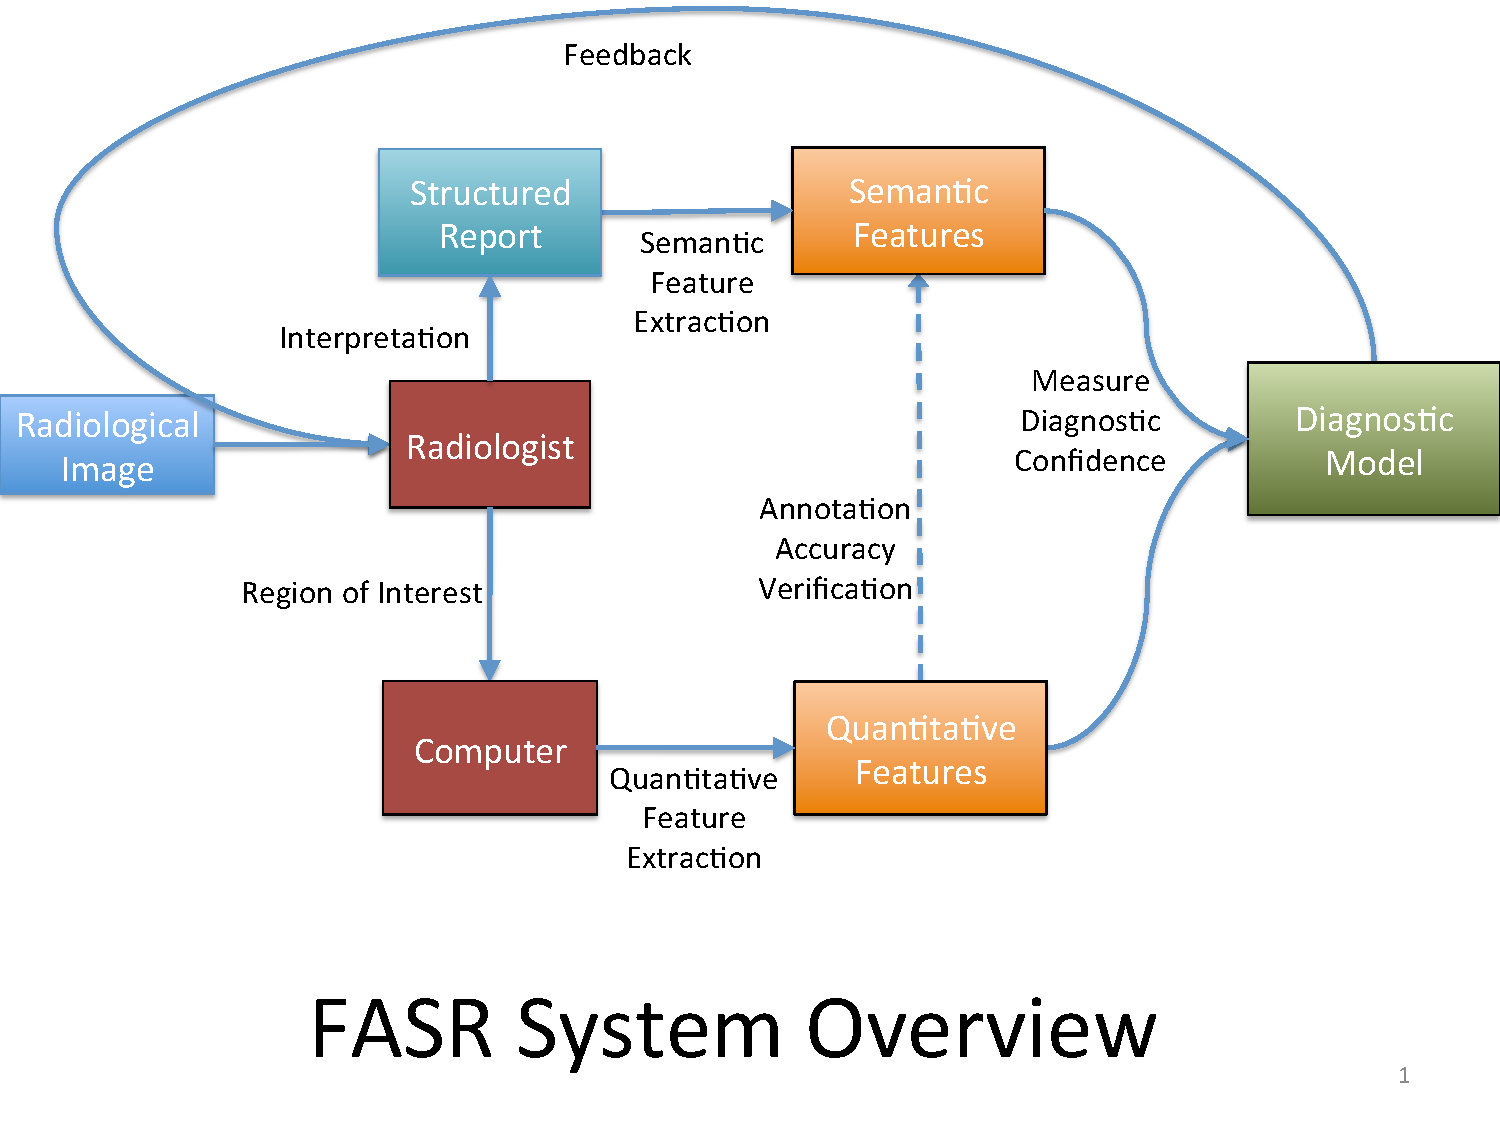
\includegraphics[width=1\linewidth]{fasr_diagram.pdf}
	\caption{Overview of the Fast Adaptive Structured Reporting (FASR) system}
	\label{fig:fasr_diagram}
\end{figure}
